
\section{Flame Graph initial: Instruments.app}

\begin{figure}[H]
  \centering
  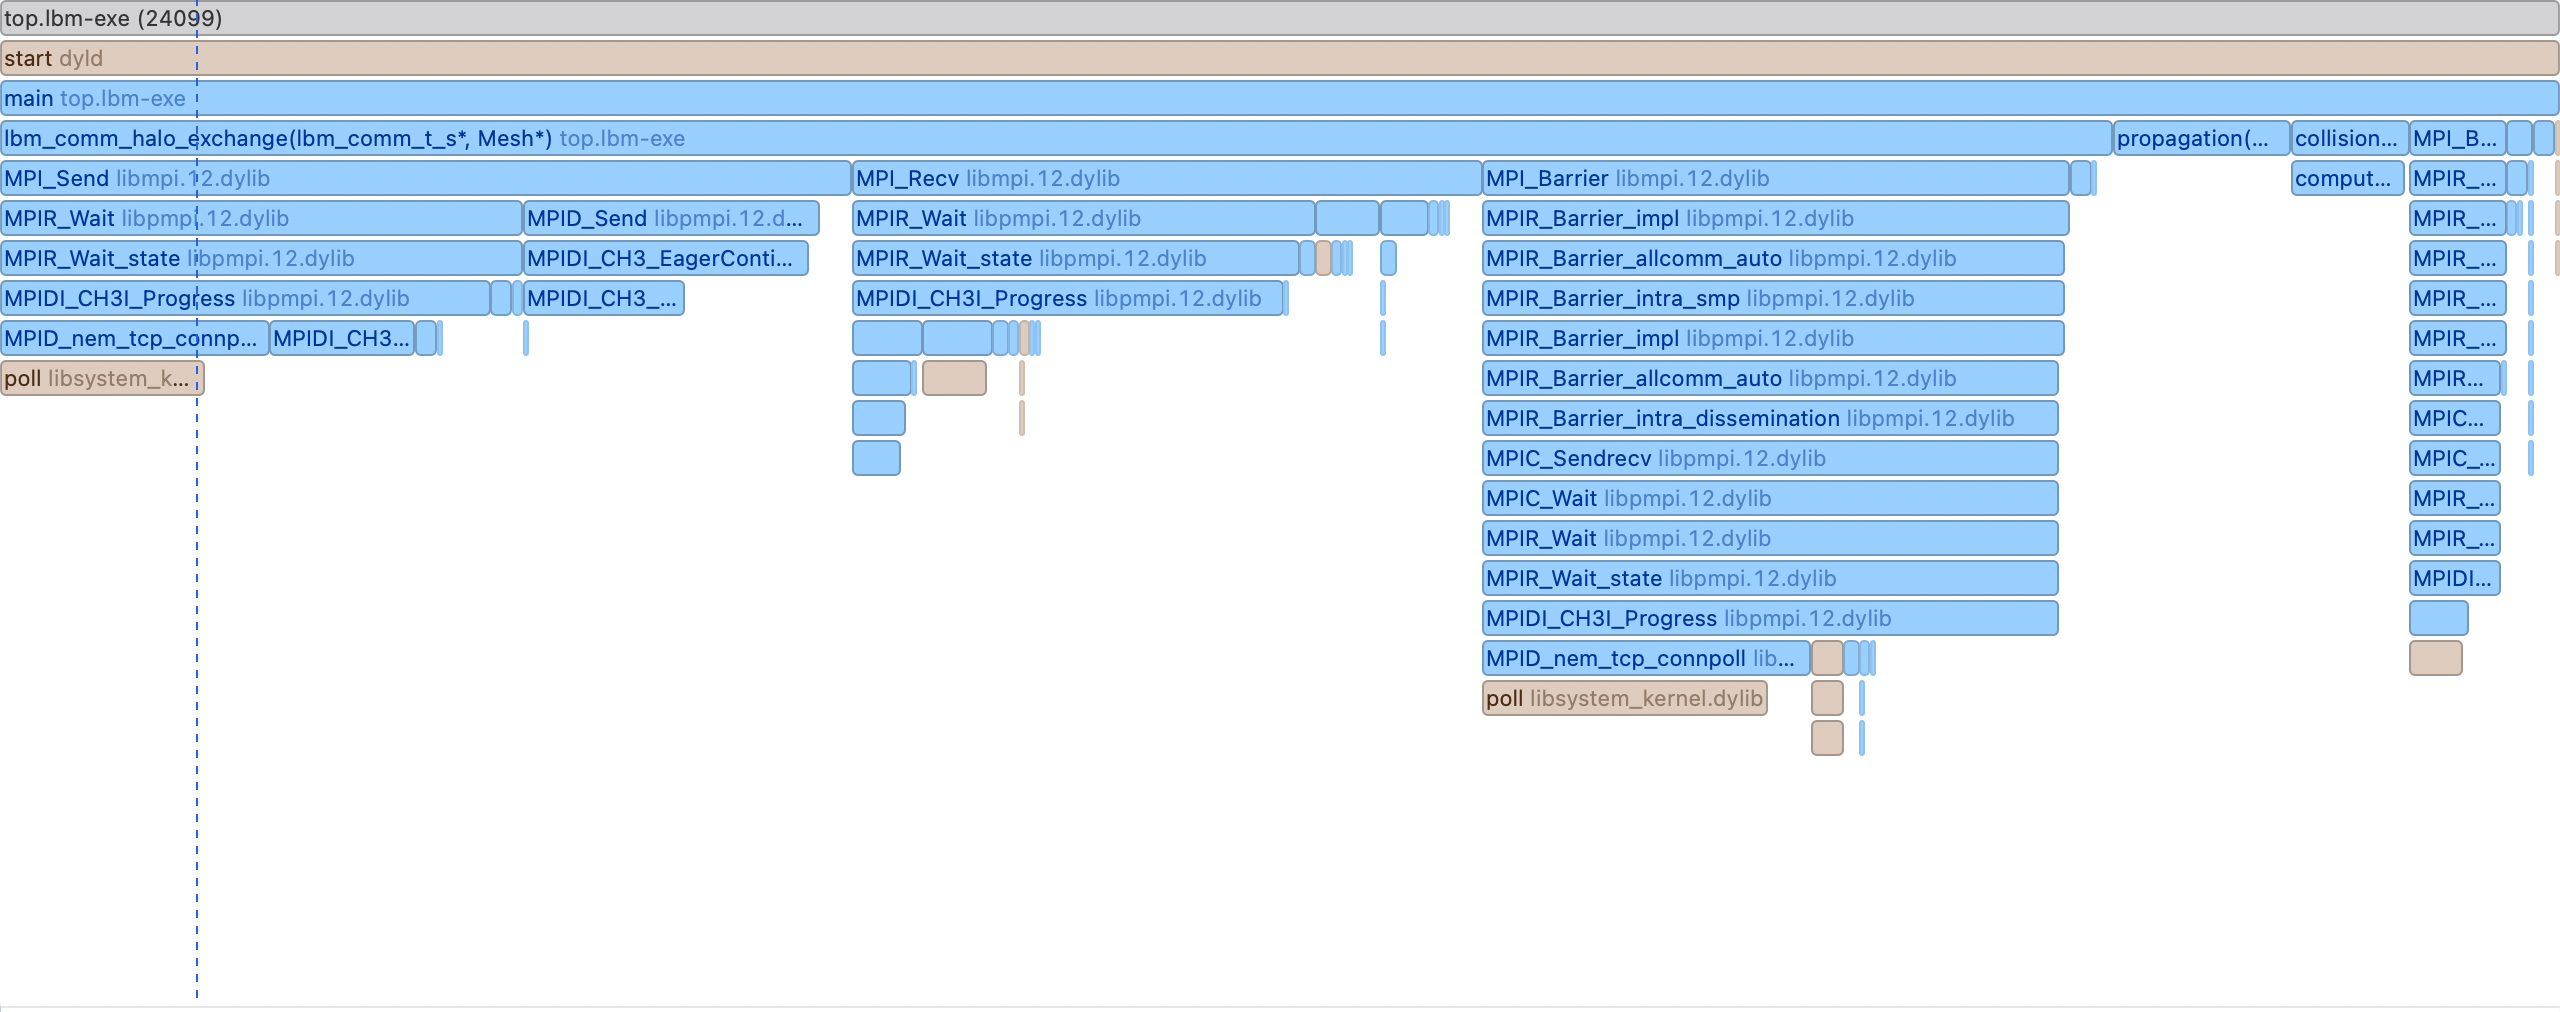
\includegraphics[scale=0.4]{graphs/flame graph 1.png}
  \label{fig:flamegraph1}
\end{figure}

\section{Fonction \textit{lbm\_comm\_halo\_exchange} initiale}
\label{section:AnnexeB}

\begin{lstlisting}[basicstyle=\tiny][language=Caml, caption=Python example]

void lbm_comm_halo_exchange(lbm_comm_t* mesh, Mesh* mesh_to_process) {
  int rank;
  MPI_Comm_rank(MPI_COMM_WORLD, &rank);

  lbm_comm_sync_ghosts_horizontal(mesh, mesh_to_process, COMM_SEND, mesh->right_id, mesh->width - 2);
  lbm_comm_sync_ghosts_horizontal(mesh, mesh_to_process, COMM_RECV, mesh->left_id, 0);
  MPI_Barrier(MPI_COMM_WORLD);

  lbm_comm_sync_ghosts_horizontal(mesh, mesh_to_process, COMM_SEND, mesh->left_id, 1);
  lbm_comm_sync_ghosts_horizontal(mesh, mesh_to_process, COMM_RECV, mesh->right_id, mesh->width - 1);
  MPI_Barrier(MPI_COMM_WORLD);

  lbm_comm_sync_ghosts_vertical(mesh_to_process, COMM_SEND, mesh->bottom_id, mesh->height - 2);
  lbm_comm_sync_ghosts_vertical(mesh_to_process, COMM_RECV, mesh->top_id, 0);
  MPI_Barrier(MPI_COMM_WORLD);

  lbm_comm_sync_ghosts_vertical(mesh_to_process, COMM_SEND, mesh->top_id, 1);
  lbm_comm_sync_ghosts_vertical(mesh_to_process, COMM_RECV, mesh->bottom_id, mesh->height - 1);
  MPI_Barrier(MPI_COMM_WORLD);

  lbm_comm_sync_ghosts_diagonal(mesh_to_process, COMM_SEND, mesh->corner_id[CORNER_TOP_LEFT], 1, 1);
  lbm_comm_sync_ghosts_diagonal(mesh_to_process, COMM_RECV, mesh->corner_id[CORNER_BOTTOM_RIGHT], mesh->width - 1,  mesh->height - 1);
  MPI_Barrier(MPI_COMM_WORLD);

  lbm_comm_sync_ghosts_diagonal(mesh_to_process, COMM_SEND, mesh->corner_id[CORNER_BOTTOM_LEFT], 1, mesh->height - 2);
  lbm_comm_sync_ghosts_diagonal(mesh_to_process, COMM_RECV, mesh->corner_id[CORNER_TOP_RIGHT], mesh->width - 1, 0);
  MPI_Barrier(MPI_COMM_WORLD);

  lbm_comm_sync_ghosts_diagonal(mesh_to_process, COMM_SEND, mesh->corner_id[CORNER_TOP_RIGHT], mesh->width - 2, 1);
  lbm_comm_sync_ghosts_diagonal(mesh_to_process, COMM_RECV, mesh->corner_id[CORNER_BOTTOM_LEFT], 0, mesh->height - 1);
  MPI_Barrier(MPI_COMM_WORLD);

  lbm_comm_sync_ghosts_diagonal(mesh_to_process, COMM_SEND, mesh->corner_id[CORNER_BOTTOM_LEFT], 1, mesh->height - 2);
  lbm_comm_sync_ghosts_diagonal(mesh_to_process, COMM_RECV, mesh->corner_id[CORNER_TOP_RIGHT], mesh->width - 1, 0);
  MPI_Barrier(MPI_COMM_WORLD);

  lbm_comm_sync_ghosts_diagonal(mesh_to_process, COMM_SEND, mesh->corner_id[CORNER_BOTTOM_RIGHT], mesh->width - 2, mesh->height - 2);
  lbm_comm_sync_ghosts_diagonal(mesh_to_process, COMM_RECV, mesh->corner_id[CORNER_TOP_LEFT], 0, 0);
  MPI_Barrier(MPI_COMM_WORLD);

  lbm_comm_sync_ghosts_horizontal(mesh, mesh_to_process, COMM_SEND, mesh->left_id, 1);
  lbm_comm_sync_ghosts_horizontal(mesh, mesh_to_process, COMM_RECV, mesh->right_id, mesh->width - 1);

  MPI_Syncall(MPI_COMM_WORLD);
}
\end{lstlisting}



\section{Flame Graph après optimisation MPI: Instruments.app}

\begin{figure}[H]
  \centering
  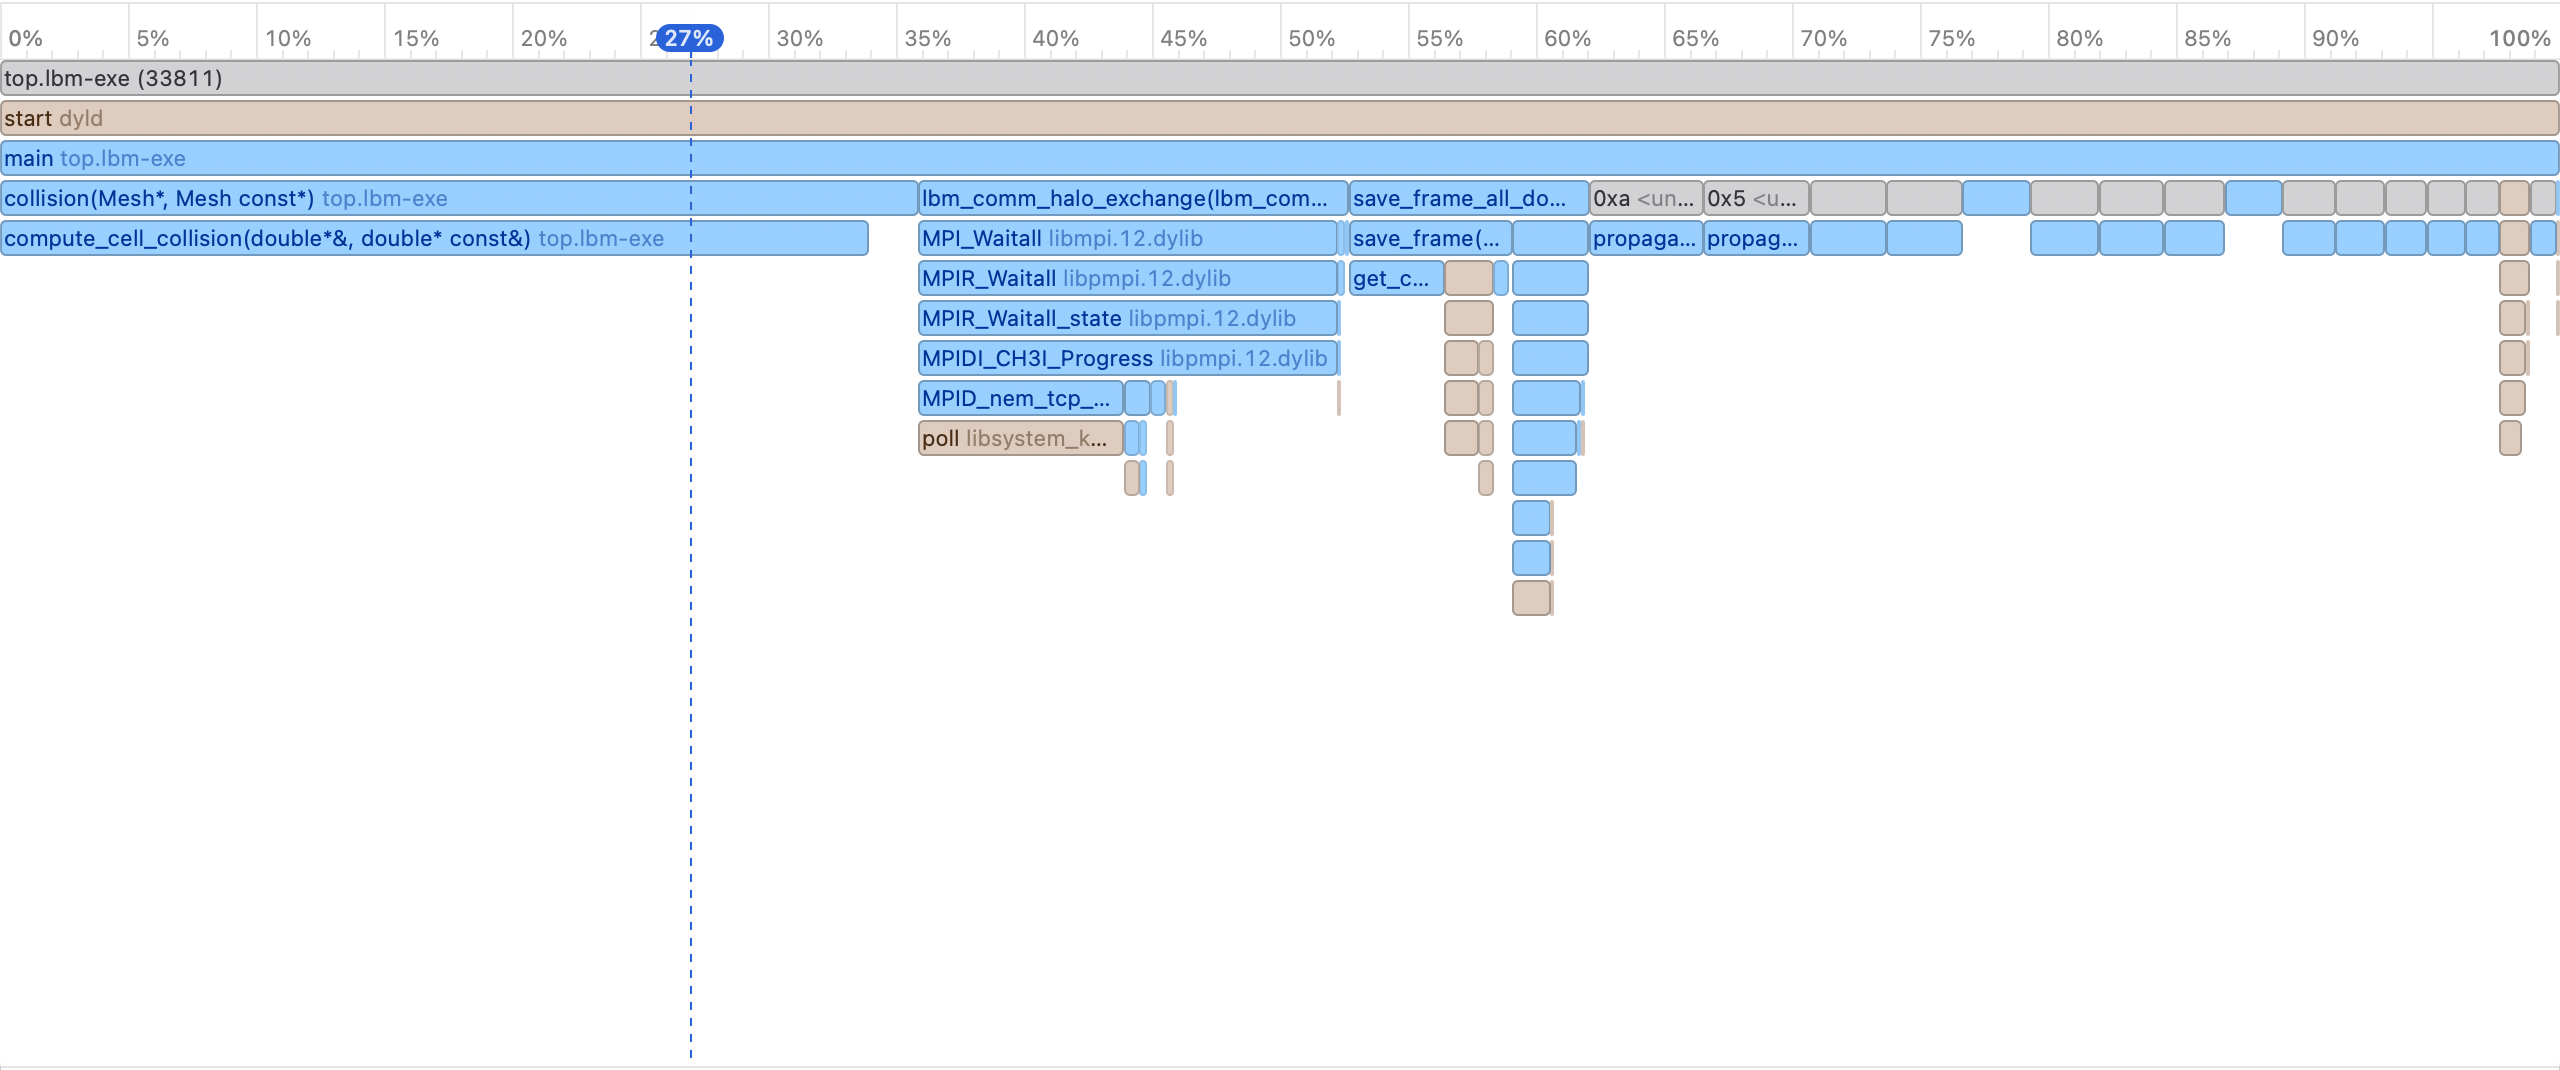
\includegraphics[scale=0.4]{graphs/flame graph 2.png}
  \label{fig:flamegraph2}
\end{figure}


\section{Comparaison version naïve et optimisée de cache-miss ratio}
\begin{figure}[H]
  \centering
  \begin{subfigure}{1.0\textwidth}
    \centering
    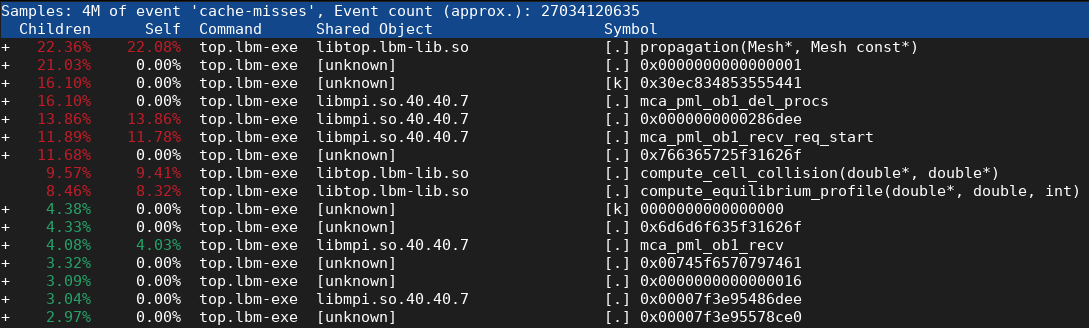
\includegraphics[scale=0.6]{graphs/miss-naive.png}
    \caption{Cache-misses version naïve}    
  \end{subfigure}
    \begin{subfigure}{1.0\textwidth}
    \centering
    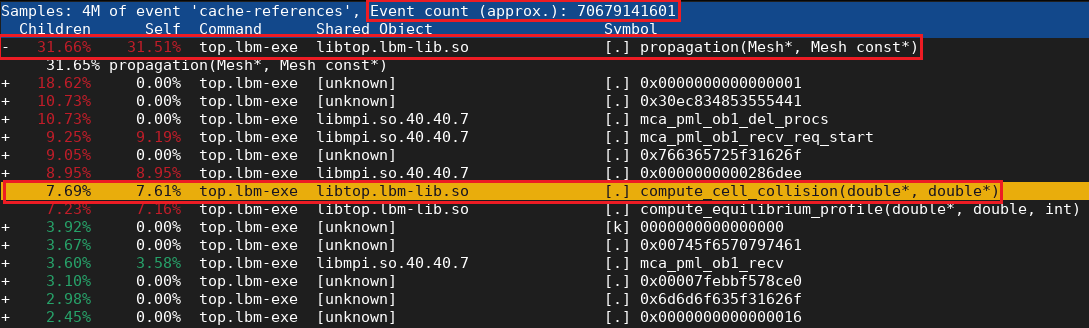
\includegraphics[scale=0.6]{graphs/ref-naive.png}
    \caption{Cache-references version naïve}
    \label{fig:perf-naive}
  \end{subfigure}
    \begin{subfigure}{1.0\textwidth}
    \centering
    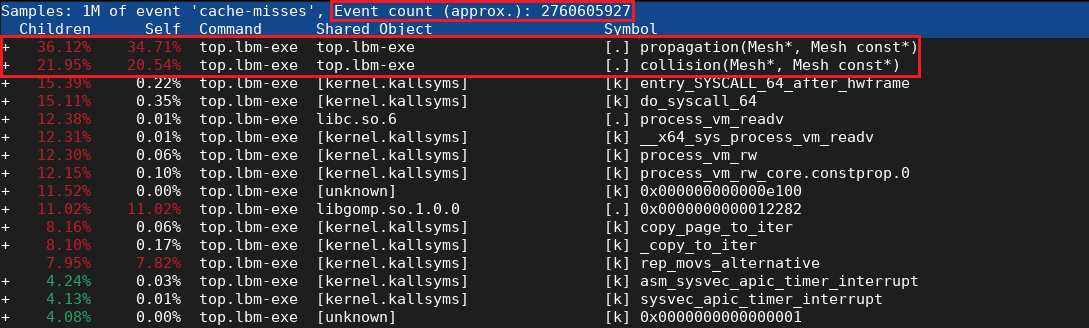
\includegraphics[scale=0.6]{graphs/miss-opti.png}
    \caption{cache-misses version optimisée}    
  \end{subfigure}
    \begin{subfigure}{1.0\textwidth}
    \centering
    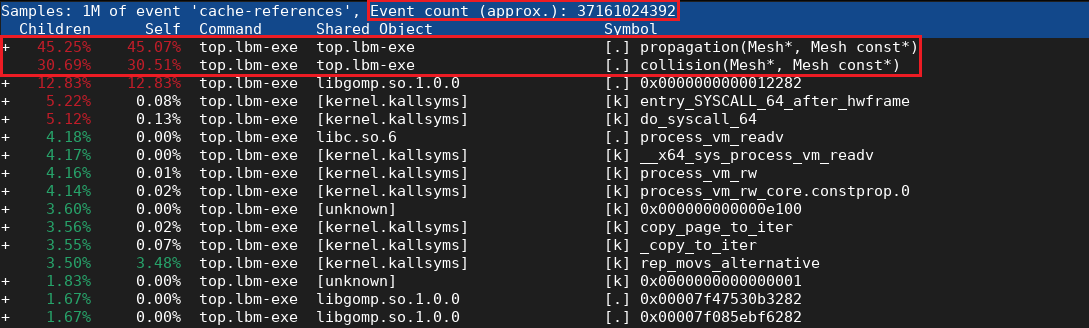
\includegraphics[scale=0.6]{graphs/ref-opti.png}
    \caption{cache-references version optimisée}
  \end{subfigure}
\end{figure}
